\chapter{Serveur}

\par Afin de garantir la bonne compréhension des différents termes techniques qui vont suivre, un lexique donnant toutes les définitions nécessaires est disponible en annexe.

\section{Architecture}

\par L’application web vise à être utilisée par des étudiants, certaines conditions de sécurité doivent donc être respectées.
 
\par Les différents programmes doivent pouvoir être lancés sur un environnement vierge indépendant et, bien sûr, isolés du serveur d’exécution afin de prévenir toute corruption de données ou problème de sécurité. Pour répondre à cette problématique, nous nous sommes tournés vers une technique encore jeune et prometteuse : la conteneurisation. Cette technique peut être utilisée via différentes technologies, celle que nous avons choisi est l’une des leaders du marché : Docker.

\subsection{Choix effectués}

\subsubsection{Choix de la conteneurisation}

\par La conteneurisation répond à nos critères d’environnement puisqu’elle permet de créer un espace propre indépendant et sans incidence sur l’environnement qui héberge le \gls{service} de chaque exécution. Grâce à cette technique, nous avons pu gérer les problèmes de sécurité et d’allocation de ressources. Nous avons choisi la conteneurisation plutôt que les machines virtuelles car elle a l’avantage d’être plus légère mais aussi plus malléable.  

\subsubsection{Choix de Docker}

\par Docker est une technologie en renouvellement permanent, nous l'avons choisie pour plusieurs raisons. \\

\par D'abord, la conteneurisation avec Docker est une option enseignée par l'Université d'Angers. Aussi, Docker est accessible et documenté. La communauté de ce dernier est très importante. Cela nous donne l’avantage de compléter nos cours en trouvant des solutions à des problèmes réguliers sur des forums, tutoriels et autres outils communautaires.


\subsection{Détails de l'architecture}

\par L’architecture du site se fait en plusieurs étapes. L'architecture actuelle est une première version qui doit être améliorée par une étude de produit plus poussée pour obtenir une architecture définitive.

\subsubsection{Architecture actuelle du site}

\begin{figure}[H]
\centering
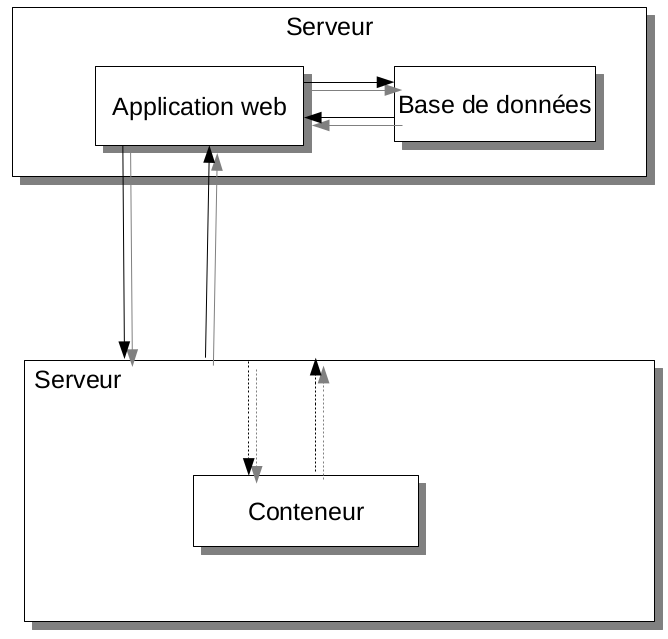
\includegraphics[width=0.5\textwidth]{./img/backend/architectureactuelle.png}
\caption{Architecture actuelle}
\end{figure}

\par La version actuelle du site utilise deux serveurs : un serveur pour l’hébergement du site et un autre pour l’exécution des différents programmes créés par les étudiants. Docker permet de créer des conteneurs éphémères sans persistance de données à partir d’une image officielle (présente dans le catalogue de docker) ou d’une image personnelle générée à partir d’un Dockerfile. Quotidiennement, les Dockerfiles sont envoyés au serveur et les images générées afin de s’assurer de la bonne version de ces dernières. Chaque langage utilisé par les étudiants possède une image unique qui lui est propre, de cette façon les images sont plus légères, plus rapides à la génération et ne possèdent que les paquets et applications nécessaires au bon fonctionnement du langage utilisé. 

\par Pour la première version du site, la communication entre l’application web et le serveur d'exécution s’effectue par SSH. Cette connexion permet l'envoi des instructions d'exécution du conteneur ainsi que les directives pour récupérer le fichier généré par l’application web qui sera à compiler. De cette manière, la gestion et la création des conteneurs est dynamique.

\subsubsection{Architecture envisagée}

\par Le client a exprimé le besoin d'utiliser plusieurs serveurs répartis sur tout le territoire français pour les exécutions des programmes. Ces serveurs seront dotés d'un système de load-balancing pour répartir les charges.
La nouvelle architecture a été pensée afin de répondre à cette nécessité, assurer une haute disponibilité et respecter la bonne utilisation des principes de Docker.

\par Dans sa version finale, l’application n’aura plus besoin d’un serveur d’hébergement. En effet, l’application entière sera conteneurisée sous forme de services : un service global pour l’exécution des conteneurs, un pour la partie web et un autre pour la base de données.

\begin{figure}[H]
\centering
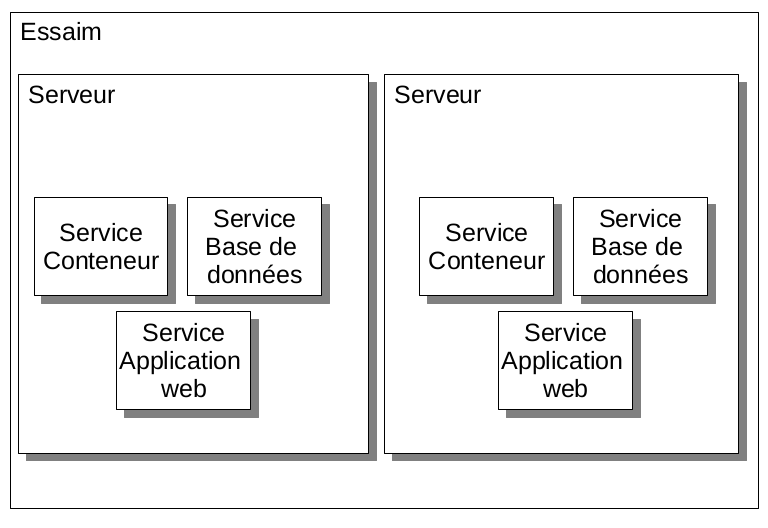
\includegraphics[width=0.6\textwidth]{./img/backend/architectureenvisagee1.png}
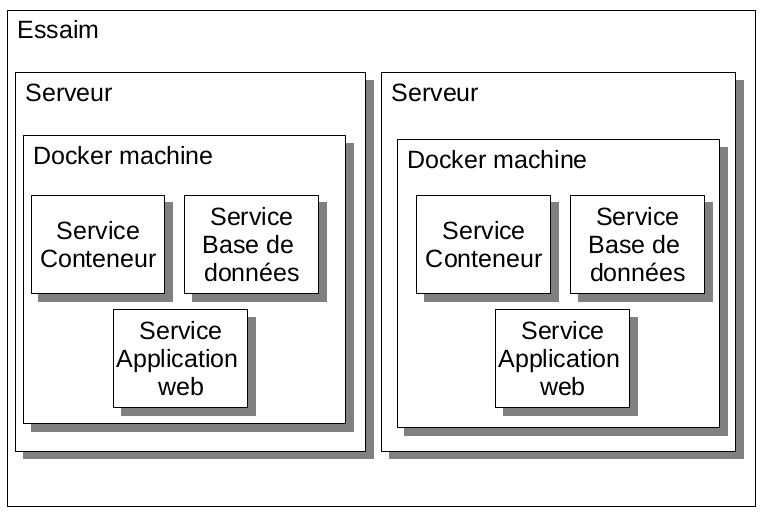
\includegraphics[width=0.6\textwidth]{./img/backend/architectureenvisagee2.png}
\caption{Architectures envisagées pour la prochaine version}
\end{figure}

\paragraph{Avantages de l'architecture envisagée}

\par L’application sera accessible en haute disponibilité. Par conséquent, les différents services pourront posséder un certain nombre de répliques et pourront gérer le load-balancing. Docker s'occupera de la synchronisation des différentes répliques de façon automatique. De plus, si l’une des répliques n’est plus actives, une autre est automatiquement créée empêchant ainsi l'application d'être impactée si un serveur venait à tomber. 

\par La transformation de l’application sous forme de service permet également de créer un Composerfile. Ce fichier permet de lancer les différents services de l’application simultanément mais également de les paramétrer. Ainsi, nous avons la certitude que tous les services sont lancés et ont la bonne configuration et, également, de garder une trace des versions.

\par De plus, un essaim Docker va être mis en place. Tous les serveurs utilisés par l’application feront partie de l’essaim, cela permettra de lier les serveurs entre eux afin de mettre en place le load-balancing.

\par La mise en place d’une telle structure soulève plusieurs questions.

\paragraph{Quelle est la configuration des différents serveurs ?} 

\par Docker est une technologie dite portable mais comme évoqué précédemment cette technologie est encore jeune et possède nombre de limites pour le moment. Pour assurer un fonctionnement identique et sans problèmes des images entre plusieurs serveurs, il faut que ces dernières aient la même configuration (même version de docker, même kernel, et même configuration système que docker pourrait exploiter, comme la prise en charge de la mémoire swap). 

\paragraph{Comment gérer la communication des conteneurs entre les différents serveurs sur des réseaux différents ?} 

\par Docker gère les répliques de services, le reverse proxy ainsi que les différents services SSH. Cependant, si les serveurs ne sont pas sur le même réseau, la communication peut vite devenir problématique. Comment assurer la sécurité ? Comment prioriser le serveur le plus proche physiquement afin de limiter la communication et avoir une vitesse maximale ? Faut-il mettre en place un serveur de communication entre les services au travers des serveurs de l’essaim ? Le principe de communication vers un conteneur à travers un service sur un essaim avec Docker reste encore assez flou à l’heure actuelle. 

\paragraph{Quel service utiliser pour mettre en place l’essaim et le load-balancing ?}

\par Actuellement, deux alternatives dominent le marché : Kubernetes et Docker swarm. Nous avons tenté de mettre en place Docker swarm mais plusieurs problèmes sont apparus. \\

\par Deux façons de faire sont possibles; soit ajouter les serveurs directement à l’essaim soit créer des \gls{dockermachine}s sur les serveurs que l’on ajoute ensuite. Les machines Docker permettent de créer un sous-réseau par hôte et d’améliorer la sécurité. Une fois les services définis et l’essaim en place, nous nous sommes rendus compte que la communication entre les services n’était pas aussi aisée que ce que l’on pouvait penser. 

\par Après avoir parcouru la documentation de Docker au sujet des essaims, nous nous sommes aperçus que la communication inter-services via l’\gls{essaim} était peu répandue et assez complexe. La mise en place d’un réseau de communication via Consul a été testée mais le temps restant ne nous a pas permis d’aller au bout de cet essai ni de l’étudier en profondeur. Ces différents problèmes ont remis en question l’utilisation de Docker swarm. Une étude des capacités de Docker swarm et de Kurbernetes est nécessaire afin de déterminer laquelle est la plus à même de répondre à nos besoins.

\paragraph{Les avantages de cette architecture}

\par L'architecture envisagée permet de définir notre application en micro-services avec une charge répartie sur plusieurs serveurs. Cela permet de rajouter des ressources au besoin. 
\par Elle permet aussi d’avoir une application en haute disponibilité : la gestion des micro-services permet, en cas de problème sur l’un d'eux, de minimiser l'ampleur de la panne mais également de répliquer sur les serveurs pour ne pas avoir de coupure si l’un des serveurs n’est plus disponible. 
\par Les conteneurs permettent d’avoir une sécurité supplémentaire à l’aide de sous-réseaux et d’environnements sans impact sur le serveur d’exécution. L’utilisation de micro-services avec un orchestrateur de \gls{conteneur}s tel que Kubernetes ou Docker swarm permet la gestion d'une grande partie de la communication et de la sécurité.   

\subsection{Problèmes rencontrés} 

\par Afin de correspondre aux besoins du client, mais aussi dans un but d'optimisation de la sécurité et de l'accessibilité, l’architecture initiale du site a dû être divisée en deux étapes : une architecture basique avec la mise en place d’un système de conteneurs et une communication temporaire. L’architecture temporaire a été pensée afin de minimiser les changements lors du passage à l’architecture envisagée. 
\par La communication a également posé des soucis, notamment lors de l’ouverture du socket SHH qui vient créer le conteneur et ne permet pas à l’étudiant d'accéder au serveur mais uniquement au conteneur.

\par Les différentes configurations de sécurité du réseau de l’Université d’Angers ont été très dérangeantes notamment lors de la génération des images grâce au \gls{dockerfile}. L’utilisation des services SSH étant bloquée, il a également été compliqué de mettre en place la connexion SSH de la première version de l’application. 